\section{Description du problème}

% But
% What you're trying to tell the audience that they don't already know (e.g. Your story.)

Un système d'exploitation moderne comme GNU/Linux est séparé en deux niveaux de
privilèges : le noyau, qui gère directement le matériel, et les applications de
l'utilisateur, qui communiquent avec le noyau par l'interface restreinte des
\emph{appels système}.

Pour assurer l'isolation, ces deux parties n'ont pas accès aux mêmes zones
mémoire (cf. figure~\ref{fig:memmap}).

\todo{figure copiée dans le chapitre isolation}

% Figure memmap {{{l
\begin{figure}
\centering
\fbox{
  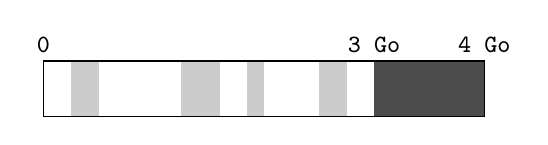
\begin{tikzpicture}
  [scale=0.7
  ,user/.style={fill=black!20}
  ,kernel/.style={fill=black!70}
  ]

  % Memory zone
  %
  % #1 - start
  % #2 - end
  % #3 - color
  \newcommand{\mzone}[3]{
    \path[#3] (#1,0) rectangle (#2,1);
  }

  % Address label
  %
  % #1 - x position
  % #2 - text
  \newcommand{\alabel}[2]{
    \path (#1,1) -- ++(0,0.3) node [pos=1] {\small \tt #2};

  }

  % exec
  \mzone{0.5}{1}{user}

  % lib
  \mzone{2.5}{3.2}{user}

  % stack
  \mzone{3.7}{4}{user}

  % stack
  \mzone{5}{5.5}{user}

  % kernel
  \mzone{6}{8}{kernel}

  % contour
  \draw (0,0) rectangle (8,1);

  \alabel{0}{0}
  \alabel{6}{3 Go}
  \alabel{8}{4 Go}

\end{tikzpicture}

}

\caption{L'espace d'adressage d'un processus. En gris clair, les zones
accessibles à tous les niveaux de privilèges : code du programme, bibliothèques,
tas, pile. En gris foncé, la mémoire du noyau, réservée au mode privilégié.}

\label{fig:memmap}
\end{figure}
% }}}

Si le code utilisateur tente d'accéder à la mémoire du noyau, une erreur sera
déclenchée. En revanche, si cette écriture est faite au sein de l'implantation
d'un appel système, il n'y aura pas d'erreur puisque le noyau a accès à toute la
mémoire : l'isolation aura donc été brisée.

Pour celui qui implante un appel système, il faut donc empêcher qu'un pointeur
passé en paramètre référence le noyau. Autrement dit, il est indispensable de
vérifier dynamiquement que la zone dans laquelle pointe le paramètre est
accessible par l'appelant\cite{hardy88confused}.

Si au contraire un tel pointeur est déréférencé sans vérification (avec
\texttt{*} ou une fonction comme \texttt{memcpy}), le code s'exécutera
correctement mais en rendant le système vulnérable, comme le montre la
figure~\ref{fig:radeon-bug}.

% Figure bug {{{
\begin{figure}
  \insertcode{radeon-buggy.c}

  \caption{Bug freedesktop.org \#29340. Le paramètre \texttt{data} provient de
    l'espace utilisateur via un appel système. Un appelant malveillant peut se
    servir de cette fonction pour lire la mémoire du noyau à travers le message
    d'erreur.}

  \label{fig:radeon-bug}
\end{figure}
% }}}

Pour éviter cela, le noyau fournit un ensemble de fonctions qui permettent de
vérifier dynamiquement la valeur d'un pointeur avant de le déréférencer. Par
exemple, dans la figure précédente, la ligne 8 aurait dû être remplacée par :

\begin{Verbatim}
copy_from_user(&value, value_ptr, sizeof(value));
\end{Verbatim}

L'analyse présentée ici permet de vérifier automatiquement et statiquement que
les pointeurs qui proviennent de l'espace utilisateur ne sont déréférencés qu'à
travers une de ces fonctions sûres.

\section{Principes de l'analyse}

% Why the audience should believe that the results you've got aren't made up or
% flawed
Le problème est modélisé de la façon suivante : on associe à chaque variable
\texttt{x} un type de données \texttt{t}, ce que l'on note \texttt{x:t}. En
plus des types présents dans le langage C, on ajoute une distinction
supplémentaire pour les pointeurs. D'une part, les pointeurs ``noyau'' (de type
\texttt{t~*}) sont créés en prenant l'adresse d'un objet présent dans le code
source. D'autre part, les pointeurs ``utilisateurs'' (leur type est noté
\texttt{t user*}) proviennent des interfaces avec l'espace utilisateur.

Il est sûr de déréférencer un pointeur noyau, mais pas un pointeur
utilisateur. L'opérateur \texttt{*} prend donc un \texttt{t *} en entrée
et produit un \texttt{t}.

Pour faire la vérification de type sur le code du programme, on a besoin de
quelques règles. Tout d'abord, les types suivent le flot de données.
C'est-à-dire que si on trouve dans le code \texttt{a = b}, \texttt{a} et
\texttt{b} doivent avoir un type compatible. Ensuite, le qualificateur
\texttt{user} est récursif : si on a un pointeur utilisateur sur une structure,
tous les champs pointeurs de la structure sont également utilisateur. Enfin, le
déréférencement s'applique aux pointeurs noyau seulement : si le code contient
l'expression \texttt{*x}, alors il existe un type \texttt{t} tel que
\texttt{x:t*} et \texttt{*x:t}.

Appliquons ces règles à l'exemple de la figure \ref{fig:radeon-bug} : on suppose
que l'interface avec l'espace utilisateur a été correctement annotée. Cela
permet de déduire que \texttt{data:void user*}. En appliquant la première règle
à la ligne 6, on en déduit que \texttt{info:struct drm\_radeon\_info user*}
(comme en C, on peut toujours convertir de et vers un pointeur sur
\texttt{void}).

Pour déduire le type de \texttt{value\_ptr} dans la ligne 7, c'est la
deuxième règle qu'il faut appliquer : le champ \texttt{value} de
la structure est de type \texttt{uint32\_t~*} mais on y accède à travers
un pointeur utilisateur, donc \texttt{value\_ptr:uint32\_t user*}.

À la ligne 8, on peut appliquer la troisième règle : à cause du déréférencement,
on en déduit que \texttt{value\_ptr:t *}, ce qui est une contradiction puisque
d'après les lignes précédentes, \texttt{value\_ptr:uint32\_t user*}.

Si la ligne 3 était remplacée par l'appel à \texttt{copy\_from\_user}, il n'y
aurait pas d'erreur de typage car cette fonction peut accepter les arguments
\texttt{(uint32\_t~*, uint32\_t user*, size\_t)}.

\section{Implantation}

Une implantation est en cours. Le code source est d'abord prétraité par
\texttt{gcc -E} puis converti en Newspeak~\cite{newspeak}, un langage destiné à
l'analyse statique. Ce traducteur peut prendre en entrée tout le langage C, y
compris de nombreuses extensions GNU utilisées dans le noyau. En particulier,
l'exemple de la figure~\ref{fig:radeon-bug} peut être analysé.

À partir de cette représentation du programme et d'un ensemble d'annotations
globales, on propage les types dans les sous-expressions jusqu'aux feuilles.

Si aucune contradiction n'est trouvée, c'est que le code respecte la propriété
d'isolation. Sinon, cela peut signifier que le code n'est pas correct, ou bien
que le système de types n'est pas assez expressif pour le code en question.

Le prototype, disponible sur \url{http://penjili.org}, fera l'objet d'une
démonstration.

\section{Conclusion}

% Recap of your story and its implications

Nous avons montré que le problème de la manipulation de pointeurs non sûrs peut
être traité avec une technique de typage. Elle est proche des analyses menées
dans CQual~\cite{pldi99} ou Sparse~\cite{TorvaldsSparse}.

% Limitations
% Why someone might doubt your story and what you've done to get rid of as much
% doubt as possible.

Plusieurs limitations sont inhérentes à cette approche : notamment, la présence
d'unions ou de \emph{casts} entre entiers et pointeurs fait échouer l'analyse.

% Extensions

Le principe de cette technique (associer des types aux valeurs puis restreindre
les opérations sur certains types) peut être repris. Par exemple, si on définit
un type ``numéro de bloc'' comme étant un nouvel alias de \texttt{int}, on peut
considérer que multiplier deux telles valeurs est une erreur.
